\documentclass[11pt]{article}
\usepackage[margin=1in]{geometry}
\usepackage{amsmath,amssymb,amsthm,mathtools}
\usepackage{graphicx}
\usepackage{microtype}
\usepackage[hidelinks]{hyperref}
\usepackage{enumitem}

\newtheorem{theorem}{Theorem}
\newtheorem{lemma}{Lemma}
\newtheorem{remark}{Remark}
\newcommand{\C}{\mathbb C}
\newcommand{\R}{\mathbb R}
\newcommand{\U}{\mathcal U}
\newcommand{\diag}{\operatorname{diag}}
\newcommand{\conv}{\operatorname{conv}}
\newcommand{\one}{\mathbf 1}

\title{A Scalar-Collision Counterexample to Exact Continuous Unitary Convexity}
\author{Candidate full answer to Question 7.2 of arXiv:2210.13309}
\date{26 August 2026}

\begin{document}
\maketitle

\begin{center}
\fbox{\parbox{0.91\textwidth}{\textbf{Status.}
Candidate full counterexample, likely valid, pending human review.  There are
diagonal self-adjoint fields $A,B\in C(X,M_3(\C))$ on a compact metric space
such that $A\prec_c B$ but $A\notin\conv(\U(B))$.  Thus Question 7.2 has a
negative answer.}}
\end{center}

\section{Source question}

Mootoo and Skoufranis ask whether, for self-adjoint continuously
diagonalizable fields $A,B\in C(X,M_n)$, continuous majorization
$A\prec_cB$ always implies exact membership
$A\in\conv(\U(B))$ \cite[Question 7.2]{MS}.  Exact membership means that
there are finitely many continuous unitary fields and one scalar probability
vector, independent of the base point.

\begin{figure}[ht]
\centering
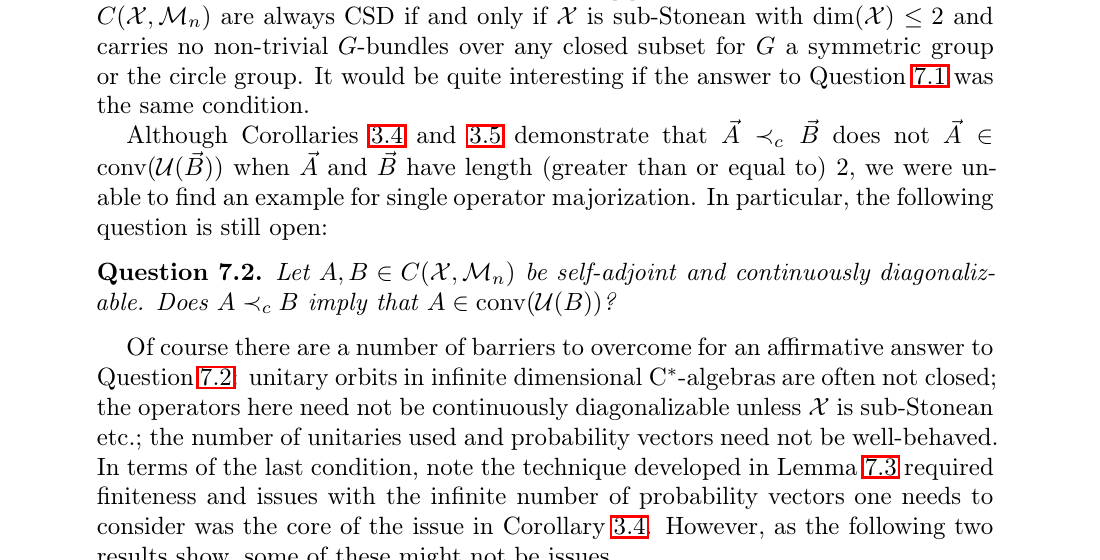
\includegraphics[width=0.96\textwidth]{source_question_crop.png}
\caption{Question 7.2 in the published source, page 20.}
\end{figure}

The source gives a counterexample for a pair of operators by exploiting the
edge between the identity and a three-cycle in the Birkhoff polytope, but
leaves the single-operator question open.  The construction below encodes the
two operators as the two first-order directions of one operator at a scalar
eigenvalue collision.

\section{Construction and result}

Let
\[
 P=\begin{bmatrix}0&1&0\\0&0&1\\1&0&0\end{bmatrix},\qquad
 \alpha(s)=\frac{1+s}{3},\qquad
 D_s=\alpha(s)I_3+(1-\alpha(s))P
\]
for $0\leq s\leq1$.  Thus $D_s$ is a nonconstant continuous path of
doubly stochastic matrices and $1/3\leq\alpha(s)\leq2/3$.

Let $K=\{z\in\R^2:\|z\|\leq1\}$, let $X=[0,1]\times K$, and write points
of $X$ as $(s,z)$, with $z=(z_1,z_2)$.  Define
\[
 b(z)=\begin{bmatrix}z_1\\z_2\\-z_1-z_2\end{bmatrix},\qquad
 B(s,z)=\diag(b(z)),\qquad
 A(s,z)=\diag(D_sb(z)).                                      \tag{1}
\]

\begin{theorem}[Negative answer to Question 7.2]\label{thm:main}
The fields $A,B\in C(X,M_3(\C))$ in \emph{(1)} are self-adjoint and
continuously diagonalizable, and $A\prec_cB$.  Nevertheless,
\[
                         A\notin\conv(\U(B)).
\]
\end{theorem}

The exceptional set is the connected interval
$[0,1]\times\{0\}$, on which $B=0$.  Away from that set, $B$ has simple
spectrum except along three lines in the $z$-disk.  The obstruction is
therefore concentrated at eigenvalue collisions, exactly outside the scope
of the simple-spectrum affirmative result.

\section{A support-rigidity lemma}

A matrix $E=[e_{ij}]\in M_3(\R)$ is \emph{unistochastic} if
$e_{ij}=|v_{ij}|^2$ for some unitary $V\in U(3)$.

\begin{lemma}[The three-cycle edge is rigid]\label{lem:rigid}
If $E$ is unistochastic and
\[
                       \operatorname{supp}(E)
                       \subseteq\operatorname{supp}(I_3+P),
\]
then $E=I_3$ or $E=P$.
\end{lemma}

\begin{proof}
Choose a unitary $V=[v_{ij}]$ with $e_{ij}=|v_{ij}|^2$.  The support
assumption gives
\[
 V=\begin{bmatrix}
       v_{11}&v_{12}&0\\
       0&v_{22}&v_{23}\\
       v_{31}&0&v_{33}
    \end{bmatrix}.
\]
The first two rows overlap in only the second column, so their orthogonality
gives $v_{12}\overline{v_{22}}=0$.  If $v_{12}=0$, the row and column norm
conditions successively force
$|v_{11}|=|v_{33}|=|v_{22}|=1$ and all other entries to vanish; hence
$E=I_3$.  If $v_{22}=0$, they instead force
$|v_{23}|=|v_{31}|=|v_{12}|=1$ and all other entries to vanish; hence
$E=P$.
\end{proof}

\section{Proof of Theorem \ref{thm:main}}

The fields in (1) are already diagonal, so they are self-adjoint and
continuously diagonalizable.  The map $(s,z)\mapsto D_s$ is a continuous
doubly stochastic witness to
\[
                         D_sb(z)=\diag(A(s,z)),
\]
and therefore $A\prec_cB$ by the definition of continuous majorization.

Suppose, toward a contradiction, that $A\in\conv(\U(B))$.  After deleting
zero coefficients, there are $m\geq1$, fixed numbers $t_j>0$ with
$\sum_jt_j=1$, and continuous unitaries $U_j:X\to U(3)$ such that
\[
             A=\sum_{j=1}^m t_j U_j^*BU_j.                  \tag{2}
\]
For $(s,z)\in X$, define
\[
 E_j(s,z)_{ik}=\left|U_j(s,z)_{ki}\right|^2.
\]
The transpose of a unitary is unitary, so every $E_j(s,z)$ is
unistochastic; it is also doubly stochastic and varies continuously.
Taking the diagonal of (2) gives
\[
             D_sb(z)=\sum_{j=1}^m t_jE_j(s,z)b(z).          \tag{3}
\]

Fix $s$ and an arbitrary $z_0\in\R^2$.  For every sufficiently small
$r>0$, substitute $z=rz_0$ into (3), divide by $r$, and let $r\downarrow0$.
Continuity yields
\[
 D_sb(z_0)=\left(\sum_{j=1}^m t_jE_j(s,0)\right)b(z_0).     \tag{4}
\]
The range of $b:\R^2\to\R^3$ is the trace-zero plane
\[
             H=\{v\in\R^3:v_1+v_2+v_3=0\}.
\]
Thus (4) says that $D_s$ and
$F_s:=\sum_jt_jE_j(s,0)$ agree on $H$.  Both matrices are doubly
stochastic, so both send $\one=(1,1,1)^T$ to $\one$.  Since
$\R^3=H\oplus\R\one$, we obtain the full matrix identity
\[
                         D_s=\sum_{j=1}^m t_jE_j(s,0).       \tag{5}
\]

Because $0<\alpha(s)<1$, the zero entries of $D_s$ are exactly the three
entries outside $\operatorname{supp}(I_3+P)$.  All $t_j$ are positive and
all entries of $E_j$ are nonnegative, so (5) forces
\[
       \operatorname{supp}(E_j(s,0))
       \subseteq\operatorname{supp}(I_3+P)
       \quad\text{for every }j,s.
\]
Lemma \ref{lem:rigid} now gives $E_j(s,0)\in\{I_3,P\}$.  For fixed $j$,
the map $s\mapsto E_j(s,0)$ is continuous from the connected interval
$[0,1]$ into the discrete two-point set $\{I_3,P\}$; hence it is constant.
The right side of (5) is therefore constant in $s$.  The left side is not,
because $\alpha(s)=(1+s)/3$.  This contradiction proves the theorem.

\section{Mechanism and scope}

The scalar collision itself erases all zeroth-order information: at $z=0$
both $A$ and $B$ vanish.  The two independent $z$-directions restore exactly
the missing information.  Passing to first order in those directions makes a
hypothetical finite unitary decomposition recover the complete matrix $D_s$
on the collision interval.  Positivity then exposes its fixed zero pattern,
and the unistochastic support lemma reduces every continuous summand to a
discrete endpoint.  Fixed scalar weights cannot reproduce a varying point on
that edge.

This also explains why a continuous single Schur--Horn choice cannot repair
the collision.  More strongly, no finite ensemble with any fixed probability
vector can repair it.  The construction uses $n=3$; the source proves the
corresponding assertion affirmatively for $n=2$.

\section{Verification and literature boundary}

The companion script \texttt{code/verify\_construction.py} checks the
doubly stochastic identities, the defining majorization equation, recovery
of $D_s$ from the two trace-zero directions plus $\one$, and the fact that
the only permutation supports contained in $I_3+P$ are $I_3$ and $P$.
The support-rigidity step for general unistochastic matrices is the exact
two-row orthogonality argument in Lemma \ref{lem:rigid}, not a numerical
inference.

Bounded exact-question, exact-title, keyword, and citation searches through
26 August 2026 found the source paper and results about \emph{closed} convex
hulls, but no later decision of Question 7.2.  A recent paper on continuity of
the Schur--Horn mapping proves local set-valued perturbation continuity
\cite{CL}; it does not supply a global continuous finite unitary ensemble and
does not address this exact-convex-hull obstruction.  The theorem here should
therefore be treated as a new candidate counterexample pending expert review.

\section{Human review recommendation}

The proof has two decisive checkpoints: verify that taking diagonals of (2)
produces the transpose-modulus-square matrices $E_j$, and verify the limiting
argument from (3) to (5).  Once (5) is obtained, positivity, Lemma
\ref{lem:rigid}, and connectedness give the contradiction directly.

\begin{thebibliography}{9}

\bibitem{MS}
X. Mootoo and P. Skoufranis,
\emph{Joint majorization in continuous matrix algebras},
J. Operator Theory \textbf{92} (2024), 413--438;
arXiv:2210.13309.

\bibitem{CL}
H. Chen and Y. Li,
\emph{On the continuity of Schur--Horn mapping},
arXiv:2407.00701, revised 4 January 2026.

\end{thebibliography}

\end{document}

